\subsection{Melihat Riwayat Penawaran}
Halaman ini hanya dapat diakses oleh pengguna yang sudah terdaftar dan sudah login. Tidak terdapat logika \textit{view} khusus pada kasus penggunaan ini. Kode sumber implementasi \textit{back-end} kasus penggunaan ini dapat dilihat pada Kode Sumber \ref{cdbe.02-04}, dan kode sumber repository terkait dapat dilihat pada Kode Sumber \ref{cdrep.02-04}.

\begin{figure}[H]
    \centering
    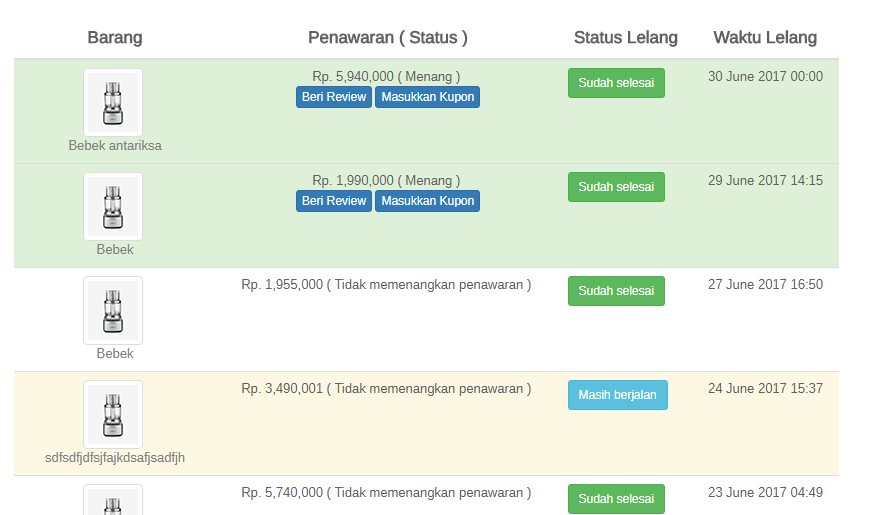
\includegraphics[width=\textwidth]{images/bab4/ui/02-04.png}
    \caption{Halaman antarmuka }
    \label{ui.02-04}
\end{figure}

\begin{lstlisting}[label=cdbe.02-04,style=php,caption=Implementasi \textit{Back-end} Kasus Penggunaan: Melihat Riwayat Penawaran]
/*	file : app/Http/Controllers/BidController*/
public function userHistory(Request $request)
{
    /*  a. Tidak ada parameter khusus
        b. Menggunakan Paginator sebagai tools bantu
        c. Terkait dengan repository BidRepository (diload dengan Dependency Injection di constructor)
        d. method : GET */

    $results = $this->bidRepository->getHistoryBid(Auth::user()->id);
    
    //Get current page form url e.g. &page=6
    $currentPage = LengthAwarePaginator::resolveCurrentPage();

    //Create a new Laravel collection from the array data
    $collection = new Collection($results);

    //Define how many items we want to be visible in each page
    $per_page = 20;

    //Slice the collection to get the items to display in current page
    $currentPageResults = $collection->slice(($currentPage-1) * $per_page, $per_page)->all();

    //Create our paginator and add it to the data array
    $data['results'] = new LengthAwarePaginator($currentPageResults, count($collection), $per_page);

    //Set base url for pagination links to follow e.g custom/url?page=6
    $data['results']->setPath($request->url());

    return view('pages.bid.bidhistory', $data);
}
\end{lstlisting}

\begin{lstlisting}[label=cdrep.02-04,style=php,caption=Implementasi \textit{Repository}: Melihat Riwayat Penawaran]
/*  file : app/Repositories/BidRepository.php */
public function getHistoryBid($id){

    /* build Query */
    $stringExecute = "SELECT MAX(b.id) as bid_id_r, b.id_item, b.id_user, u.name, i.name,
                        i.bid_status, b.bid_time, b.win_status, MAX(b.price_bid) as price_bid ,MAX(b.bid_timestamp)
                        FROM bids b
                        left JOIN users u ON u.id = b.id_user
                        left JOIN items i ON i.id = b.id_item
                        WHERE b.id_user = ".Auth::user()->id."
                        GROUP BY b.id_item, b.id_user, u.name, i.name, i.bid_status, b.bid_time,
                        b.win_status
                        ORDER BY bid_id_r DESC;";
    
    $result = DB::select($stringExecute);

    /* return result */
    return $result;
}
\end{lstlisting}


